\documentclass[dvipdfmx]{beamer}
\usetheme{metropolis}
\usepackage[T1]{fontenc}
\usepackage{lmodern}
\usepackage{tikz}
% \usepackage{gnuplot-lua-tikz}
\usepackage{empheq}
\usepackage{ulem}
\usepackage{amsmath, amsthm}
\usepackage{mathtools}
\usepackage{cases}
\usepackage{ascmac}
\usepackage{bbm}
\usepackage{capt-of}
\usepackage{siunitx}
\usefonttheme{professionalfonts} 
\setbeamertemplate{navigation symbols}{} 

% \theoremstyle{definition}
% \newtheorem{dfn}{Definition}
% \newtheorem{thm}{Theorem}
% \newtheorem{prop}{Proposition}
% \newtheorem{cor}{Corollary}

\theoremstyle{remark}
\newtheorem*{rem*}{Remark}

% \numberwithin{equation}{section}

%---------------------------------- mytitle---------------------------------------
\title{ポテンシャル逆問題の新たな設定と\\バブリング法による数値計算}
\date{}
% \author{\textsf{守田龍平}}
\author{守田龍平 \and 今川真城 \and 磯祐介}
\institute{京都大学大学院情報学研究科先端数理科学専攻}
%=============================================================================
%=============================================================================
\begin{document}

\begin{frame}
  \maketitle
\end{frame}

\begin{frame}{研究の概要}
  % \footnote{佐々木晶,『惑星内部構造』,地震,61巻特集号,2009, 285-296.}
  \underline{ポテンシャルは観測量として有効では?}

  \begin{figure}
    \centering
    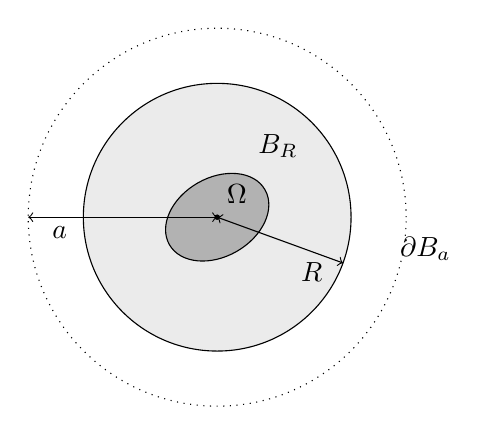
\begin{tikzpicture}
      \filldraw [fill=black!8!] (0,0)circle[radius=1.7];
      \filldraw [fill=black!30!] (-0,0)circle[x radius=0.7,y radius=0.5,rotate=30];
      \draw(0,0.3)node[right]{$\Omega$};
      \draw(0.4,0.9)node[right]{$B_R$};
      \draw(2.2,-0.4)node[right]{$\partial B_a$};
      \draw[<->](0,0)--({1.7*cos(-20)},{1.7*sin(-20)});
      \draw[<->](0,0)--(-2.4,0);
      \draw (1.2,-0.7)node{$R$};
      \draw (-2,-0.2)node{$a$};
      \fill (0,0) circle (1pt); 
      \draw[dotted] (0,0)circle[radius=2.4];
    \end{tikzpicture}
    \caption{惑星の二層モデルの人工衛星による推定}
  \end{figure}


\end{frame}

\begin{frame}{ポテンシャルの定義と性質}
  領域$D\subset \mathbb{R}^3$上の密度関数$\mu(x)$に対し,ポテンシャルを定義する.
  \begin{align}\label{teigi}
    U^{\mu}(x) := \int_{D}E(x-y)\mu(y)dy,\quad x\in\mathbb{R}^3. \nonumber
  \end{align}
  但し,$E$はLaplace方程式の基本解であり,
  \[
    E(x) = \frac{1}{4\pi}\frac{1}{|x|}
  \]
  である.

  $\mu\in L_c^\infty$のとき,ポテンシャル$U^\mu$には次の性質がある.
  \begin{itemize}
    \item $x\in\mathbb{R}^3$で連続
    \item (超関数の意味で)$\overline{D}^c$で調和
  \end{itemize}

  % \begin{figure}
    % \centering
    % \begin{tikzpicture}
      % % \filldraw [fill=black!10!] (0,0)circle[radius=1.6];
      % \draw (0,0)circle[radius=1.6];
      % \filldraw [fill=black!20!] (-0.1,0.2)circle[x radius=0.7,y radius=0.5,rotate=30];
      % \draw(0,0.3)node[right]{$\Omega$};
      % \draw(0.4,0.7)node[right]{$B_{r_0}$};
      % \draw[<->](0,0)--(-1.6,0);
      % \draw (-0.9,0)node[below]{$r_0$};
      % \fill (0,0) circle (1pt); 
    % \end{tikzpicture}
  % \end{figure}

\end{frame}


\begin{frame}{二層モデル}
  二層モデルを考える.

  領域$\Omega\subset B_R$とする.
  密度関数が$\mu_e=\mathbbm{1}_{B_R}+\rho\mathbbm{1}_{\Omega}$とすると,
  $\partial B_a$上で観測するポテンシャル$U^{\mu_e}$は次の通り.
  \begin{align*}
    U^{\mu_e}(x) = U^{\mathbbm{1}_{B_R}}(x) + U^{\rho\mathbbm{1}_\Omega}(x),\quad x\in\partial B_a.
  \end{align*}
  これより,$\Omega$のポテンシャルを$\partial B_a$で観測することが可能である.
  \begin{align*}
    U^{\rho\mathbbm{1}_\Omega}(x) = U^{\mu_e}(x) - U^{\mathbbm{1}_{B_R}}(x),\quad x\in\partial B_a.
  \end{align*}

  \begin{columns}
    \centering 
    \begin{column}{0.48\textwidth}
      \centering
      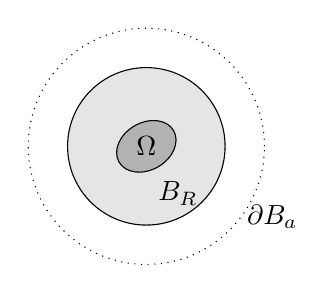
\begin{tikzpicture}
        \filldraw [fill=black!10!] (0,0)circle[radius=1.0];
        \filldraw [fill=black!30!] (-0,0)circle[x radius=0.4,y radius=0.3,rotate=30];
        \draw[dotted] (0,0)circle[radius=1.5];
        \draw(-0,0)node{$\Omega$};
        % \draw[<->](0,0)--(-0.6,0);
        % \draw[<->](0,0)--({1.6*cos(-20)},{1.6*sin(-20)});
        \draw (0.4,-0.6)node{$B_R$};
        \draw (1.6,-0.9)node{$\partial B_a$};
        % \fill (0,0) circle (1pt); 
      \end{tikzpicture}
    \end{column} 
    \hspace{-2cm}

    $\rightarrow$

    % \hspace{-1cm}
    \begin{column}{0.48\textwidth}
      \centering
      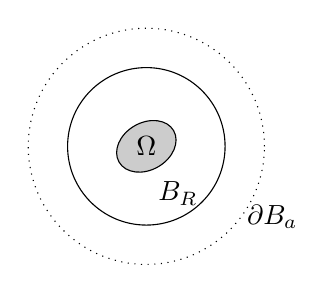
\begin{tikzpicture}
        \filldraw [fill=black!0!] (0,0)circle[radius=1.0];
        \filldraw [fill=black!20!] (-0,0)circle[x radius=0.4,y radius=0.3,rotate=30];
        \draw[dotted] (0,0)circle[radius=1.5];
        \draw(-0,0)node{$\Omega$};
        % \draw[<->](0,0)--(-0.6,0);
        % \draw[<->](0,0)--({1.6*cos(-20)},{1.6*sin(-20)});
        \draw (0.4,-0.6)node{$B_R$};
        \draw (1.6,-0.9)node{$\partial B_a$};
        % \fill (0,0) circle (1pt); 
      \end{tikzpicture}
    \end{column}

  \end{columns}


\end{frame}


\begin{frame}{ポテンシャル逆問題}
  (測地学における)ポテンシャル逆問題
  \footnote{
    G.Anger, 
    \textit{Inverse Problems in Differential Equations},
    Plenum Press,
    1990.
  }
  では,観測面$\partial B_a$上で重力$g$を観測し,物体の形状$\Omega$を回復する.
  つまり,境界条件
    \[
      \nabla U^{\rho\mathbbm{1}_\Omega} = \overrightarrow{g} \quad \mathrm{on} \quad \partial B_a \nonumber
    \]
  をみたす$\Omega$を求める.
  \begin{itembox}[c]{新たな設定}
  ポテンシャルの減衰は重力に比べて弱いので,
  \[
    U^{\rho\mathbbm{1}_\Omega} = p \quad \mathrm{on} \quad \partial B_a
  \]
  を境界条件とする.
  \end{itembox}
\end{frame}

\begin{frame}{離散化した境界条件}
  先ほどの問題設定における境界条件は
  \begin{itemize}
    \item 重力観測
    \[
      \nabla U^{\rho\mathbbm{1}_\Omega} = \overrightarrow{g} \quad \mathrm{on} \quad \partial B_a
    \]
  
    \item ポテンシャル観測
    \[
      U^{\rho\mathbbm{1}_\Omega} = p \quad \mathrm{on} \quad \partial B_a
    \]
  \end{itemize}
  だった.
  しかし,実際には観測できるのは観測面$\partial B_a$上の有限個の地点$\{A_n\}_{n=1}^N$なので,
  各$n$に対し
  \begin{itemize}
    \item 重力観測
    \[
      \nabla U^{\rho\mathbbm{1}_\Omega} = \overrightarrow{g_n} \quad \mathrm{on} \quad A_n
    \]
  
    \item ポテンシャル観測
    \[
      U^{\rho\mathbbm{1}_\Omega} = p_n \quad \mathrm{on} \quad A_n
    \]
  \end{itemize}
  という離散化した境界条件を考えることにする.
\end{frame}

\begin{frame}{数値計算概要(1/2)}
  (離散版)境界条件は次の通り.
  \begin{itemize}
    \item 重力観測
    \[
      \nabla U^{\rho\mathbbm{1}_\Omega} = \overrightarrow{g_n} \quad \mathrm{on} \quad A_n
    \]
  
    \item ポテンシャル観測
    \[
      U^{\rho\mathbbm{1}_\Omega} = p_n \quad \mathrm{on} \quad A_n 
    \]
  \end{itemize}
領域回復のアルゴリズムは次の2つのアルゴリズムから成る.
数値計算は主として
Zidarov
\footnote{D.Zidarov, \textit{Inverse Gravimetric Problem in Geoprospecting and Geodesy}, Elsevier, 1990.}
に倣う.
\begin{enumerate}
  \item 観測点上の重力またはポテンシャルを有限個の質点で近似 \\
  \item バブリング法(質量を均す)
\end{enumerate}

\ 

\end{frame}

\begin{frame}{数値計算概要(2/2)}
  \begin{figure}
    \centering
    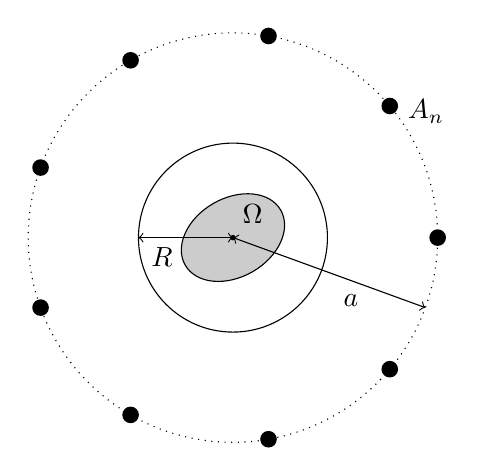
\begin{tikzpicture}
      \filldraw [fill=black!20!] (-0,0)circle[x radius=0.7,y radius=0.5,rotate=30];
      \draw(0,0.3)node[right]{$\Omega$};
      \draw(2.1,1.6)node[right]{$A_n$};
      \draw[<->](0,0)--(-1.2,0);
      \draw[<->](0,0)--({2.6*cos(-20)},{2.6*sin(-20)});
      \draw (-0.9,0)node[below]{$R$};
      \draw (1.5,-0.8)node{$a$};
      \fill (0,0) circle (1pt); 
      \draw (0,0)circle[radius=1.2];
      \draw[dotted] (0,0)circle[radius=2.6];

      \fill ({2.6*cos(0)},{2.6*sin(0}) circle (3pt); 
      \fill ({2.6*cos(40)},{2.6*sin(40}) circle (3pt); 
      \fill ({2.6*cos(80)},{2.6*sin(80}) circle (3pt); 
      \fill ({2.6*cos(120)},{2.6*sin(120}) circle (3pt); 
      \fill ({2.6*cos(160)},{2.6*sin(160}) circle (3pt); 
      \fill ({2.6*cos(200)},{2.6*sin(200)}) circle (3pt); 
      \fill ({2.6*cos(240)},{2.6*sin(240}) circle (3pt); 
      \fill ({2.6*cos(280)},{2.6*sin(280}) circle (3pt); 
      \fill ({2.6*cos(320)},{2.6*sin(320}) circle (3pt); 
    \end{tikzpicture}
    \caption{ポテンシャル逆問題の数値計算概要}
  \end{figure}

\end{frame}


\begin{frame}{観測した重力を有限個の質点で近似する}

  観測点を$\{A_n\}_{n=1}^N\subset \partial B_a$とする.

  質点の系を$(X,M)=(X_1,\dots X_K,\dots ,M_1,\dots M_K)$で表す.
  コスト関数$J_G$を
  \begin{gather*}
    J_G(X, M) = \frac{1}{N}\sum_{n=1}^N\left|\nabla U^{\rho\mathbbm{1}_\Omega}(A_n) - G_K(A_n;X,M)\right|^2,\\ 
    \quad G_K(A_n;X,M) = \frac{1}{4\pi}\sum_{k=1}^K\frac{M_k(A_n-X_k)}{|A_n-X_k|^3}
  \end{gather*}
  として定め,$J_G$を(局所)最小化する.
\end{frame}

\begin{frame}{観測したポテンシャルを有限個の質点で近似する}
  観測点を$\{A_n\}_{n=1}^N\subset \partial B_a$とする.

  質点の系を$(X,M)=(X_1,\dots X_K,\dots ,M_1,\dots M_K)$で表す.
  コスト関数$J_P$を
  \begin{gather*}
    J_P(X, M) = \frac{1}{N}\sum_{n=1}^N(U^{\rho\mathbbm{1}_\Omega}(A_n) - P_K(A_n;X,M))^2, \\
    P_K(A_n;X,M) = \frac{1}{4\pi}\sum_{k=1}^K \frac{M_k}{|A_n-X_k|}
  \end{gather*}
  として定め,$J_P$を(局所)最小化する.
\end{frame}

\begin{frame}{数値計算 最適化アルゴリズムの設定}
観測面$\partial B_a$上等間隔に$N$個の観測地点$\{A_n\}_{n=1}^N$をとる.

初期値とする質点は$\partial B_{a}$上等間隔に$K$個の初期地点$\{X_k^{(0)}\}_{k=1}^K$とし,
各質点の質量は $M_k^{(0)} = \rho\pi R^2/K$ とする.


\begin{rem*}
  人工衛星による重力の分解能は高々$10^{-5}\si{m/s^2}$であり,
  \footnote{宮原伐折羅,『国土地理院の重力観測の展望-測定技術と重力基準の将来像』,国土地理院時報,2018, No.~131, 95-108.}
  原子時計によるポテンシャル観測の分解能は高々$10^{-4}\si{m^2/s^2}$である.
  \footnote{野崎京三,『原子時計をセンサーとした重力ポテンシャル計の可能性』,応用地質技術年報,2011, No.~30, 65-71.}
\end{rem*}

\end{frame}

% \begin{frame}{バブリング法 (Partial Mass Scattering)}
  % 質点の系を密度$\rho$の物体に均す.

  % 領域$B_{R}$を幅$h$のメッシュで切り,
  % 質点$(X_k,M_k)$を最近傍格子点$\widetilde{X}_k=(ih, jh)$に移動する.
  % $\widetilde{M}_{i,j}=M_k$とする.

  % $\Delta \widetilde{M}_{i,j} = \widetilde{M}_{i,j}-\rho h^2 > \varepsilon$とき,
  % \begin{gather*}
    % \widetilde{M}_{i,j}^{(1)}=\rho h^2-\varepsilon, \\
    % \widetilde{M}_{i\pm 1,j}^{(1)}=\widetilde{M}_{i\pm 1,j}+\frac{1}{4}(\Delta \widetilde{M}_{i,j}+\varepsilon),\quad
    % \widetilde{M}_{i,j\pm 1}^{(1)}=\widetilde{M}_{i,j\pm 1}+\frac{1}{4}(\Delta \widetilde{M}_{i,j}+\varepsilon)\quad
  % \end{gather*}
  % として更新する.
  % \begin{columns}
    % \centering 
    % \begin{column}{0.48\textwidth}
      % \centering
        % \begin{tikzpicture}
          % \draw [dotted,thin] (-1.25,-1.25) grid [step=1] (1.25,1.25);
          % \fill [red] (0,0) circle (3pt); 
          % \draw (0.35,0.40) circle (3pt); 
          % \fill (0.35,0.40) circle (2pt); 

          % \fill (1,0) circle (3pt);
          % \fill (1,1) circle (3pt);
          % \fill (0,1) circle (3pt);
          % \fill (-1,1) circle (3pt);
          % \fill (-1,0) circle (3pt);
          % \fill (-1,-1) circle (3pt);
          % \fill (0,-1) circle (3pt);
          % \fill (1,-1) circle (3pt);

          % \draw(0.7,0.7)node{$M_{i,j}$};
          % \draw[->](0.25,0.30)--(0.1,0.1);
        % \end{tikzpicture}
        % \captionof{figure}{格子点に移動}
    % \end{column} 
    % \hspace{-1cm}

    % \hspace{-1cm}
    % \begin{column}{0.48\textwidth}
      % \centering
        % \begin{tikzpicture}
          % \draw [dotted,thin] (-1.25,-1.25) grid [step=1] (1.25,1.25);
          % \fill [red] (0,0) circle (3pt); 
          % \fill [blue] (-1,0) circle (3pt); 
          % \fill [blue] (1,0) circle (3pt); 
          % \fill [blue] (0,1) circle (3pt); 
          % \fill [blue] (0,-1) circle (3pt); 

          % \fill (1,1) circle (3pt); 
          % \fill (1,-1) circle (3pt); 
          % \fill (-1,1) circle (3pt); 
          % \fill (-1,-1) circle (3pt); 

          % \draw(0.4,0.3)node{$\widetilde{M}_{i,j}$};
          % \draw[->](0.2,0)--(0.5,0);
          % \draw[->](0,0.2)--(0,0.5);
          % \draw[->](-0.2,0)--(-0.5,0);
          % \draw[->](0,-0.2)--(0,-0.5);
        % \end{tikzpicture}
        % \captionof{figure}{質量の拡散}
    % \end{column}

  % \end{columns}


% \end{frame}

% \begin{frame}{数値計算 バブリング法の設定}
  % 格子点$(ih,jh)$に乗っている質量を$\widetilde{M}_{i,j}$で表す.
  % $\Delta \widetilde{M}_{i,j} = \widetilde{M}_{i,j}-\rho h^2 > \varepsilon$とき,
  % \[
    % \widetilde{M}_{i,j}^{(1)}=\rho h^2-\varepsilon
  % \]
  % で更新する.
  % メッシュ幅$h$は$10^{-2}$,パラメータ$\varepsilon$は$10^{-5}$とした.
  % \begin{figure}
    % \begin{tikzpicture}
      % \draw [dotted,thin] (-2.2,-2.2) grid (2.2,2.2);
      % \fill (-2,2) circle (3pt); 
      % \fill (-1,2) circle (3pt); 
      % \fill (0,2) circle (3pt); 
      % \fill (1,2) circle (3pt); 
      % \fill (2,2) circle (3pt); 

      % \fill (-2,1) circle (3pt); 
      % \fill (-1,1) circle (3pt); 
      % \fill (0,1) circle (3pt); 
      % \fill (1,1) circle (3pt); 
      % \fill (2,1) circle (3pt); 

      % \fill (-2,0) circle (3pt); 
      % \fill (-1,0) circle (3pt); 
      % \fill (0,0) circle (3pt); 
      % \fill (1,0) circle (3pt); 
      % \fill (2,0) circle (3pt); 

      % \fill (-2,-1) circle (3pt); 
      % \fill (-1,-1) circle (3pt); 
      % \fill (0,-1) circle (3pt); 
      % \fill (1,-1) circle (3pt); 
      % \fill (2,-1) circle (3pt); 

      % \fill (-2,-2) circle (3pt); 
      % \fill (-1,-2) circle (3pt); 
      % \fill (0,-2) circle (3pt); 
      % \fill (1,-2) circle (3pt); 
      % \fill (2,-2) circle (3pt); 

      % % \draw (1.8,1.3) circle (3pt); 
      % % \fill (1.8,1.3) circle (2pt); 

      % \fill [red] (2,1) circle (3pt); 
      % \fill [red] (-1,-1) circle (3pt); 

      % \fill [blue] (-2,-1) circle (3pt); 
      % \fill [blue] (-1,-2) circle (3pt); 
      % \fill [blue] (-1,0) circle (3pt); 
      % \fill [blue] (0,-1) circle (3pt); 

      % \fill [blue] (1,1) circle (3pt); 
      % \fill [blue] (2,0) circle (3pt); 
      % \fill [blue] (2,2) circle (3pt); 
      % % \fill [blue] (3,1) circle (3pt); 

      % \draw[->](-0.8,-1)--(-0.2,-1);
      % \draw[->](-1.2,-1)--(-1.8,-1);
      % \draw[->](-1,-0.8)--(-1,-0.2);
      % \draw[->](-1,-1.2)--(-1,-1.8);

      % \draw[-](2.2,1)--(2.4,1);
      % \draw[->](1.8,1)--(1.2,1);
      % \draw[->](2,1.2)--(2,1.8);
      % \draw[->](2,0.8)--(2,0.2);
    % \end{tikzpicture}
    % \caption{バブリング法}
  % \end{figure}
% \end{frame}

\begin{frame}{数値計算 目標の確認}

  観測半径$a$を変えたとき,最適化法+バブリング法による領域$\Omega$の形状回復への影響を調査する.
  \begin{figure}
    \centering
    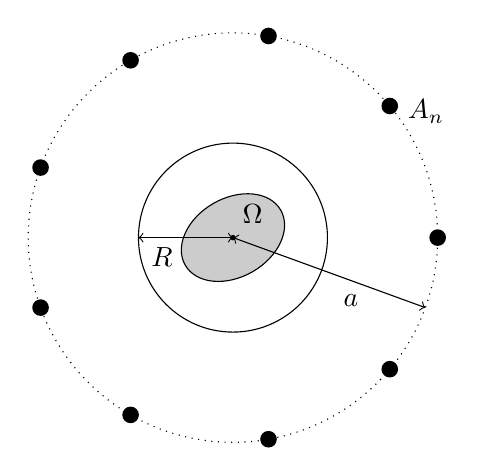
\begin{tikzpicture}
      \filldraw [fill=black!20!] (-0,0)circle[x radius=0.7,y radius=0.5,rotate=30];
      \draw(0,0.3)node[right]{$\Omega$};
      \draw(2.1,1.6)node[right]{$A_n$};
      \draw[<->](0,0)--(-1.2,0);
      \draw[<->](0,0)--({2.6*cos(-20)},{2.6*sin(-20)});
      \draw (-0.9,0)node[below]{$R$};
      \draw (1.5,-0.8)node{$a$};
      \fill (0,0) circle (1pt); 
      \draw (0,0)circle[radius=1.2];
      \draw[dotted] (0,0)circle[radius=2.6];

      \fill ({2.6*cos(0)},{2.6*sin(0}) circle (3pt); 
      \fill ({2.6*cos(40)},{2.6*sin(40}) circle (3pt); 
      \fill ({2.6*cos(80)},{2.6*sin(80}) circle (3pt); 
      \fill ({2.6*cos(120)},{2.6*sin(120}) circle (3pt); 
      \fill ({2.6*cos(160)},{2.6*sin(160}) circle (3pt); 
      \fill ({2.6*cos(200)},{2.6*sin(200)}) circle (3pt); 
      \fill ({2.6*cos(240)},{2.6*sin(240}) circle (3pt); 
      \fill ({2.6*cos(280)},{2.6*sin(280}) circle (3pt); 
      \fill ({2.6*cos(320)},{2.6*sin(320}) circle (3pt); 
    \end{tikzpicture}
    \caption{ポテンシャル逆問題の数値計算概要}
  \end{figure}

\end{frame}




% \begin{frame}{円板の回復}
  % 原点中心半径$1$の円板の回復を試みる.

  % 質点の数$K=1$,観測点$N=3$とし,観測半径$R$を変えてその影響について数値計算する.
  % 最適化にはNewton法を用いた.
  % コスト関数$J_P, J_G$を$0$とする$(X_1,M_1)$が存在し,いずれの場合も$X_1=0, M_1=\pi$に限られている.

  % \begin{figure}
    % \centering
    % \begin{tikzpicture}
      % \filldraw [fill=black!10!] (0,0) circle [radius=0.5];
      % \fill (0,0) circle (1pt); 
      % \draw[dotted] (0,0)circle[radius=1];
      % \draw[<->](0,0)--(-1,0);
      % \draw[<->](0,0)--({2*cos(-20)},{2*sin(-20)});
      % \draw(1.5,0)node[below]{$R$};
      % \draw(-0.7,0)node[above]{$r_0$};
      % \draw (0,0)circle[radius=2];
      % \fill (2,0) circle (3pt); 
      % \fill ({2*cos(0)},{2*sin(0}) circle (3pt); 
      % \fill ({2*cos(120)},{2*sin(120}) circle (3pt); 
      % \fill ({2*cos(240)},{2*sin(240}) circle (3pt); 
    % \end{tikzpicture}
  % \end{figure}

% \end{frame}



\begin{frame}{数値計算例:楕円形のコアの回復}
  惑星の半径$R=2$とする.
  長半径$\sqrt{2}$,短半径$1$,密度$\rho=10$の楕円の回復を試みる.
  最適化にはLevenberg-Marquardt法を用いた.

  \begin{figure}
    \centering
    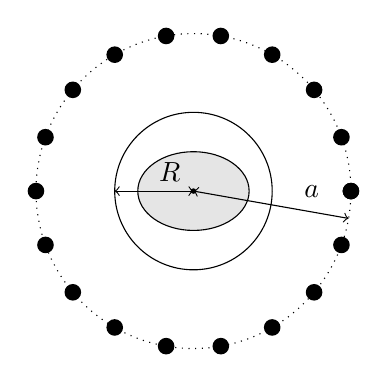
\begin{tikzpicture}
      % \filldraw[fill=black!10!] ({-0.25*sqrt(3)},-0.25) -- ++(0:{0.5*sqrt(3)}) -- ++(120:{0.5*sqrt(3)}) -- cycle;
      \filldraw [fill=black!10!] (0,0)circle[x radius=0.707,y radius=0.5,rotate=0];
      \fill (0,0) circle (1pt); 
      \draw (0,0)circle[radius=1];
      \draw[<->](0,0)--(-1,0);
      \draw[<->](0,0)--({2*cos(-10)},{2*sin(-10)});
      \draw(1.5,0)node{$a$};
      \draw(-0.3,0)node[above]{$R$};
      \draw[dotted] (0,0)circle[radius=2];
      \fill (2,0) circle (3pt); 
      \fill ({2*cos(0)},{2*sin(0}) circle (3pt); 
      \fill ({2*cos(20)},{2*sin(20}) circle (3pt); 
      \fill ({2*cos(40)},{2*sin(40}) circle (3pt); 
      \fill ({2*cos(60)},{2*sin(60}) circle (3pt); 
      \fill ({2*cos(80)},{2*sin(80}) circle (3pt); 
      \fill ({2*cos(100)},{2*sin(100}) circle (3pt); 
      \fill ({2*cos(120)},{2*sin(120}) circle (3pt); 
      \fill ({2*cos(140)},{2*sin(140}) circle (3pt); 
      \fill ({2*cos(160)},{2*sin(160}) circle (3pt); 
      \fill ({2*cos(180)},{2*sin(180}) circle (3pt); 
      \fill ({2*cos(200)},{2*sin(200}) circle (3pt); 
      \fill ({2*cos(220)},{2*sin(220}) circle (3pt); 
      \fill ({2*cos(240)},{2*sin(240}) circle (3pt); 
      \fill ({2*cos(260)},{2*sin(260}) circle (3pt); 
      \fill ({2*cos(280)},{2*sin(280}) circle (3pt); 
      \fill ({2*cos(300)},{2*sin(300}) circle (3pt); 
      \fill ({2*cos(320)},{2*sin(320}) circle (3pt); 
      \fill ({2*cos(340)},{2*sin(340}) circle (3pt); 
    \end{tikzpicture}
  \end{figure}

\end{frame}

\begin{frame}{数値計算例:楕円形のコアの回復 重力観測}
  質点の数$K=30$,観測点数$N=90$とする.
  $a$は観測半径である.
  \begin{columns}
    \begin{column}{0.38\columnwidth}
      \centering
      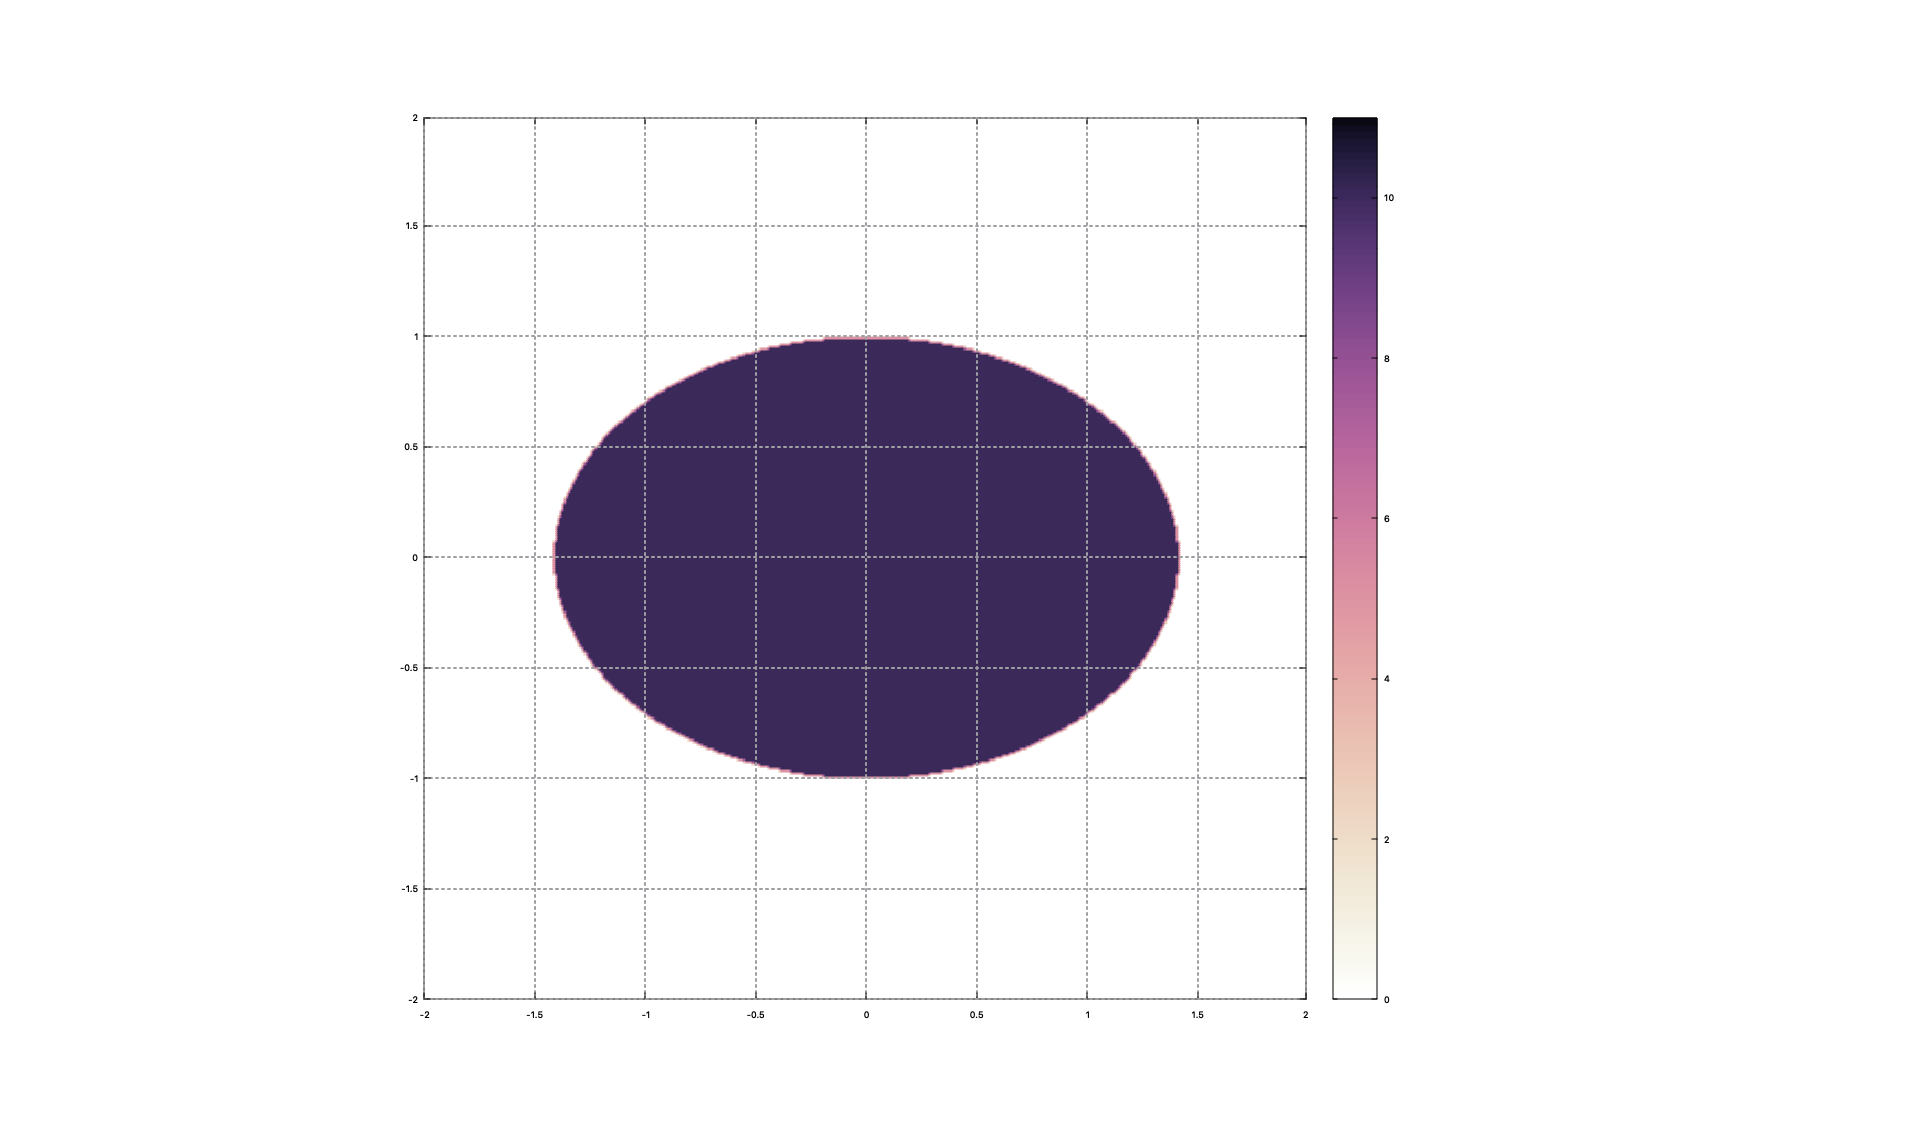
\includegraphics[width=4cm]{fig/elliptic.png}
      \captionof{figure}{厳密解}
    \end{column}
    \hspace{-1cm}
    \begin{column}{0.38\columnwidth}
      \centering
      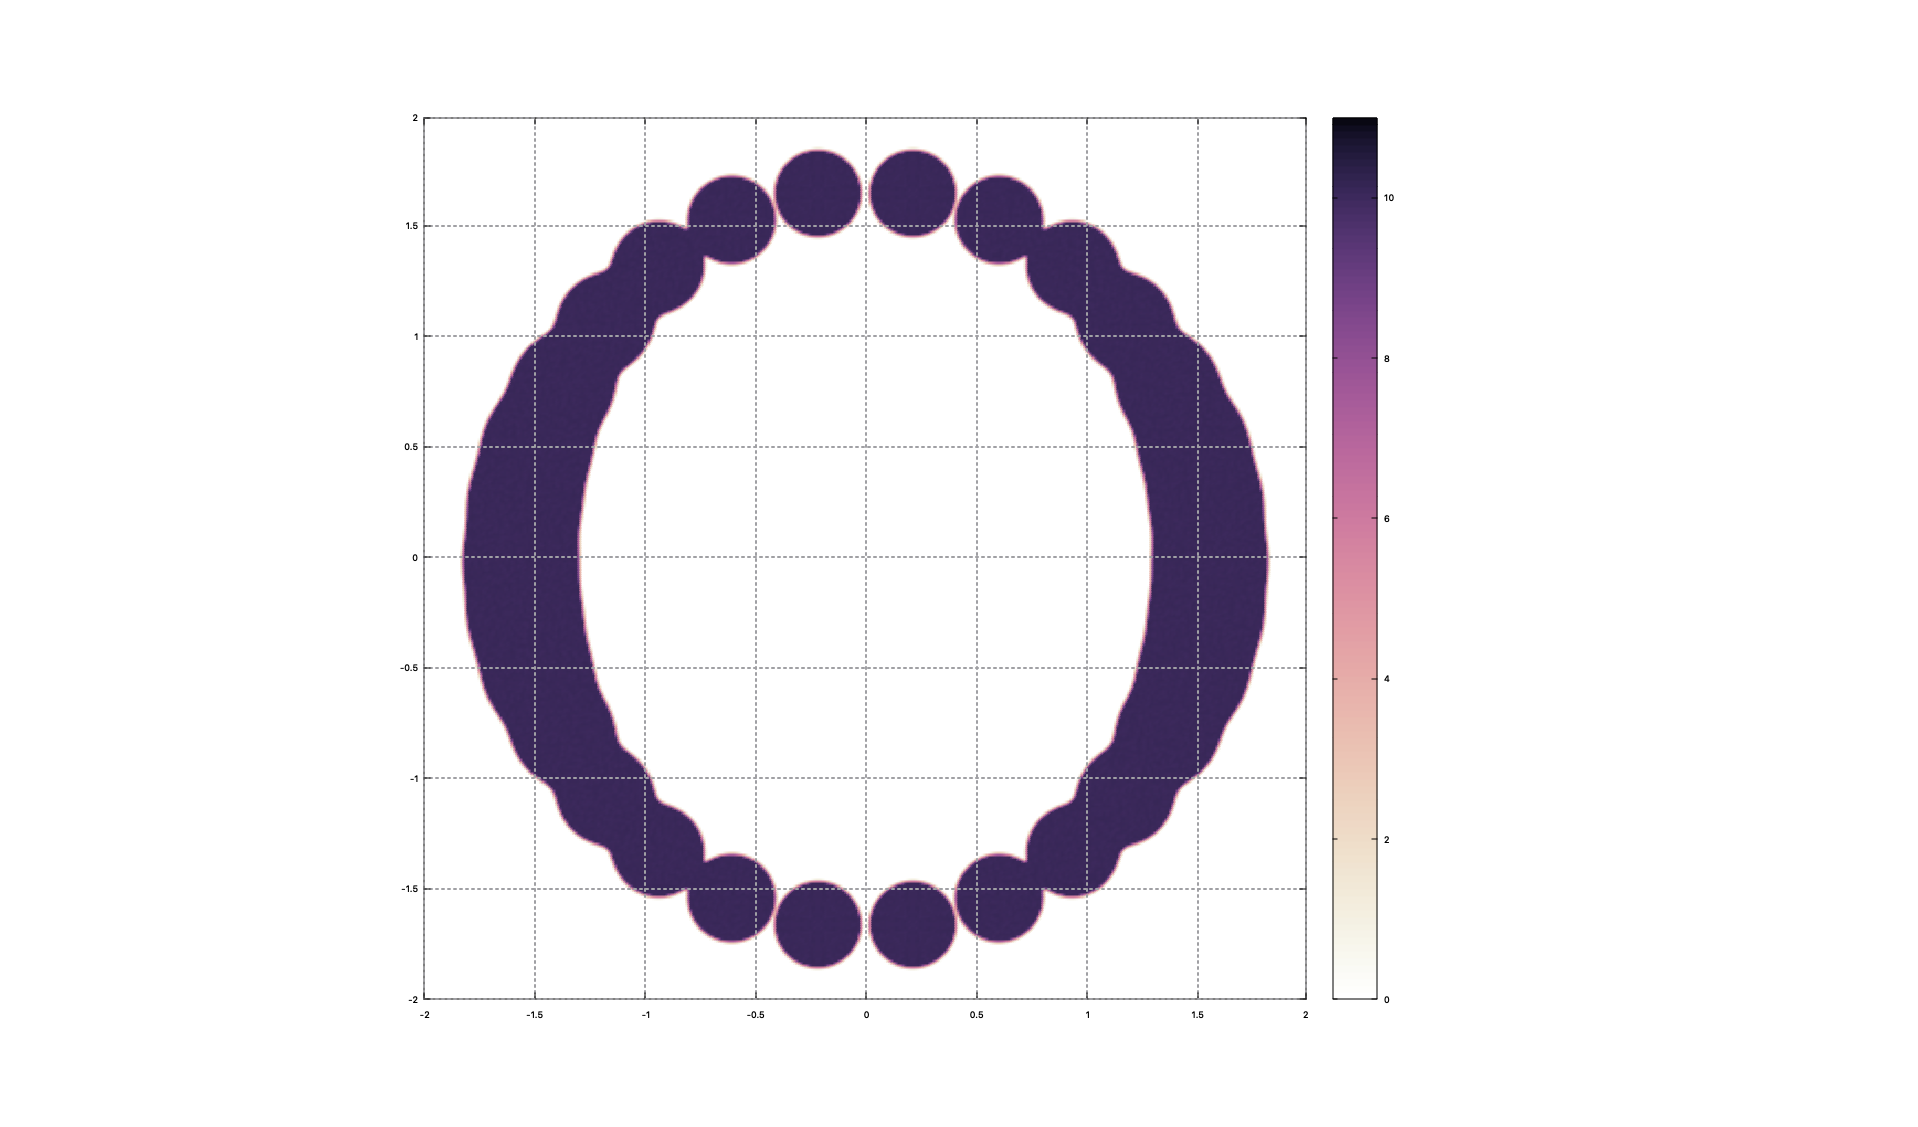
\includegraphics[width=4cm]{fig/GR4N90K30E2.png}
      \captionof{figure}{$a=4$}
    \end{column}
  \end{columns}

  \begin{columns}
    \begin{column}{0.38\columnwidth}
      \centering
      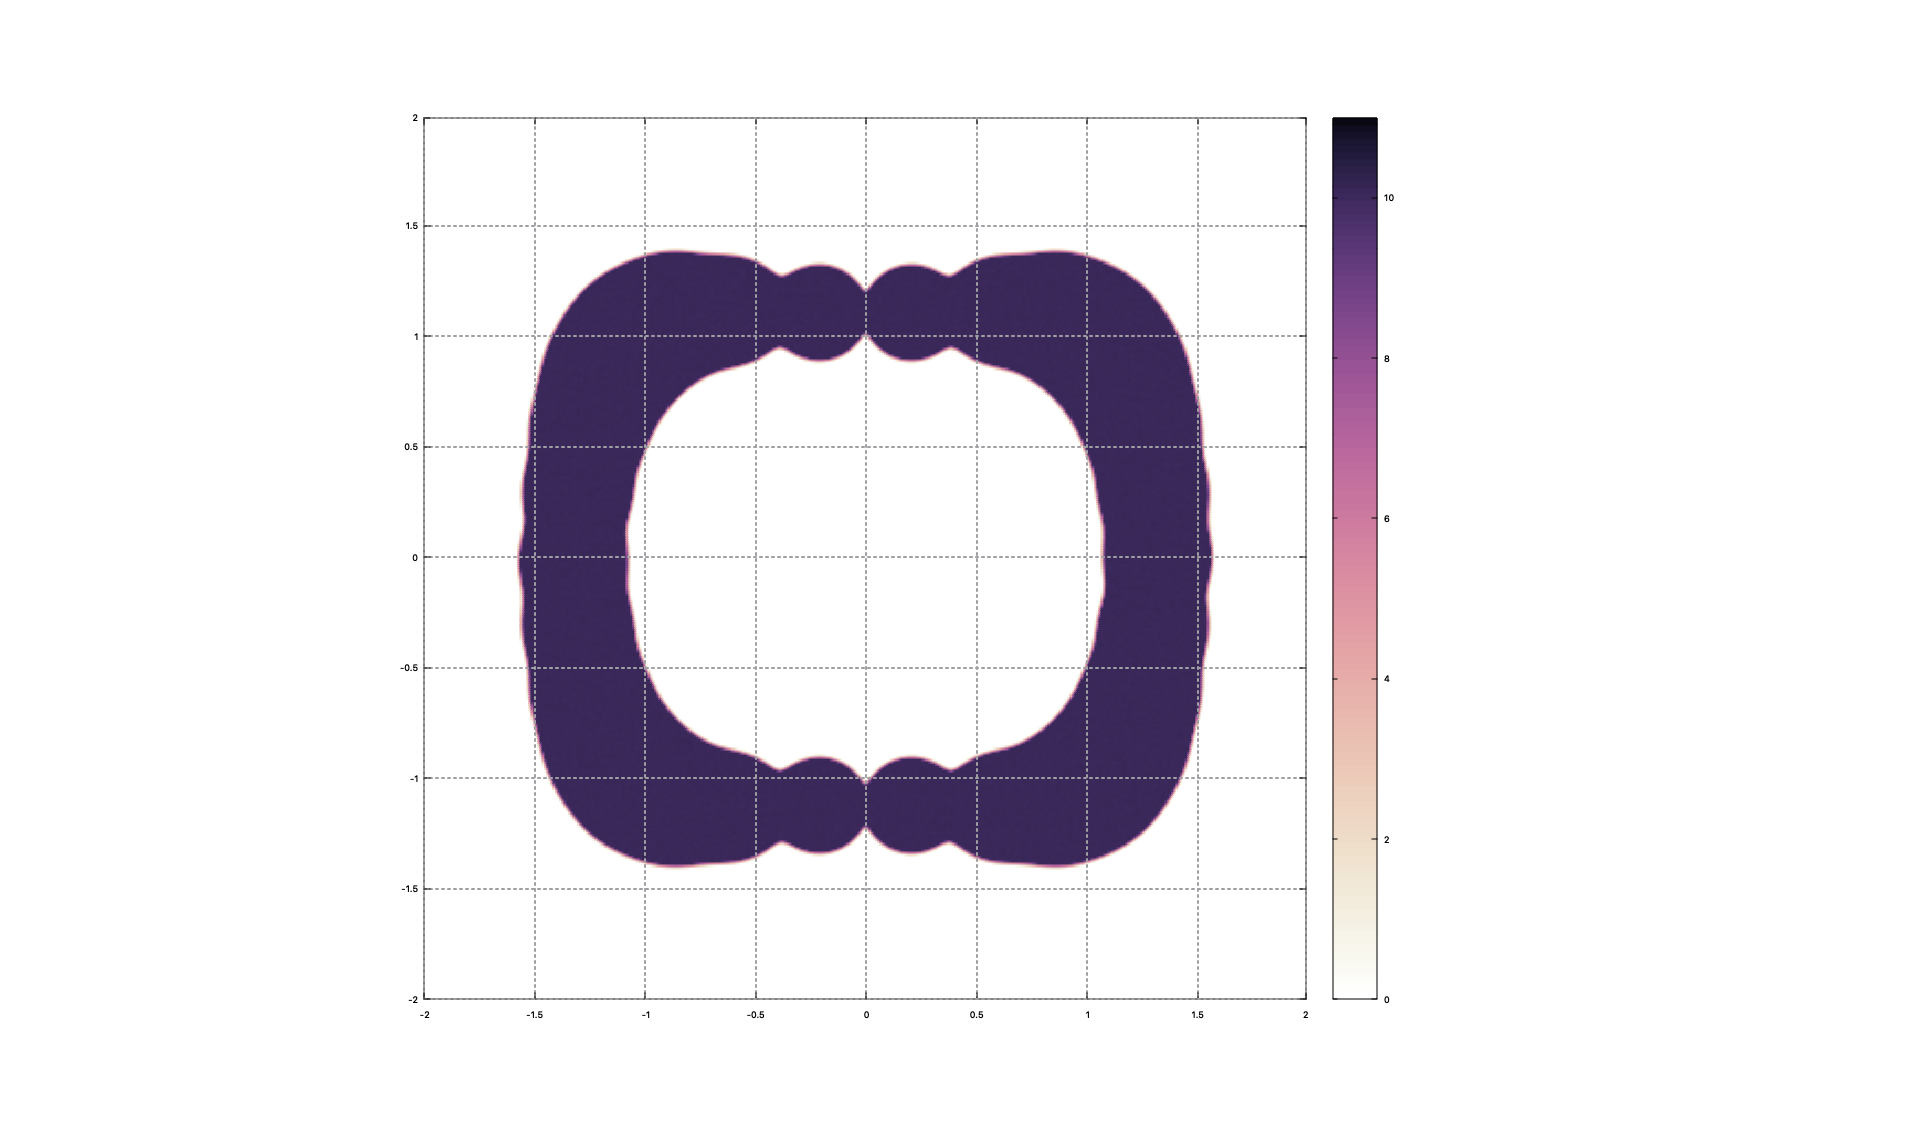
\includegraphics[width=4cm]{fig/GR10N90K30E2.png}
      \captionof{figure}{$a=10$}
    \end{column}
    \hspace{-1cm}
    \begin{column}{0.38\columnwidth}
      \centering
      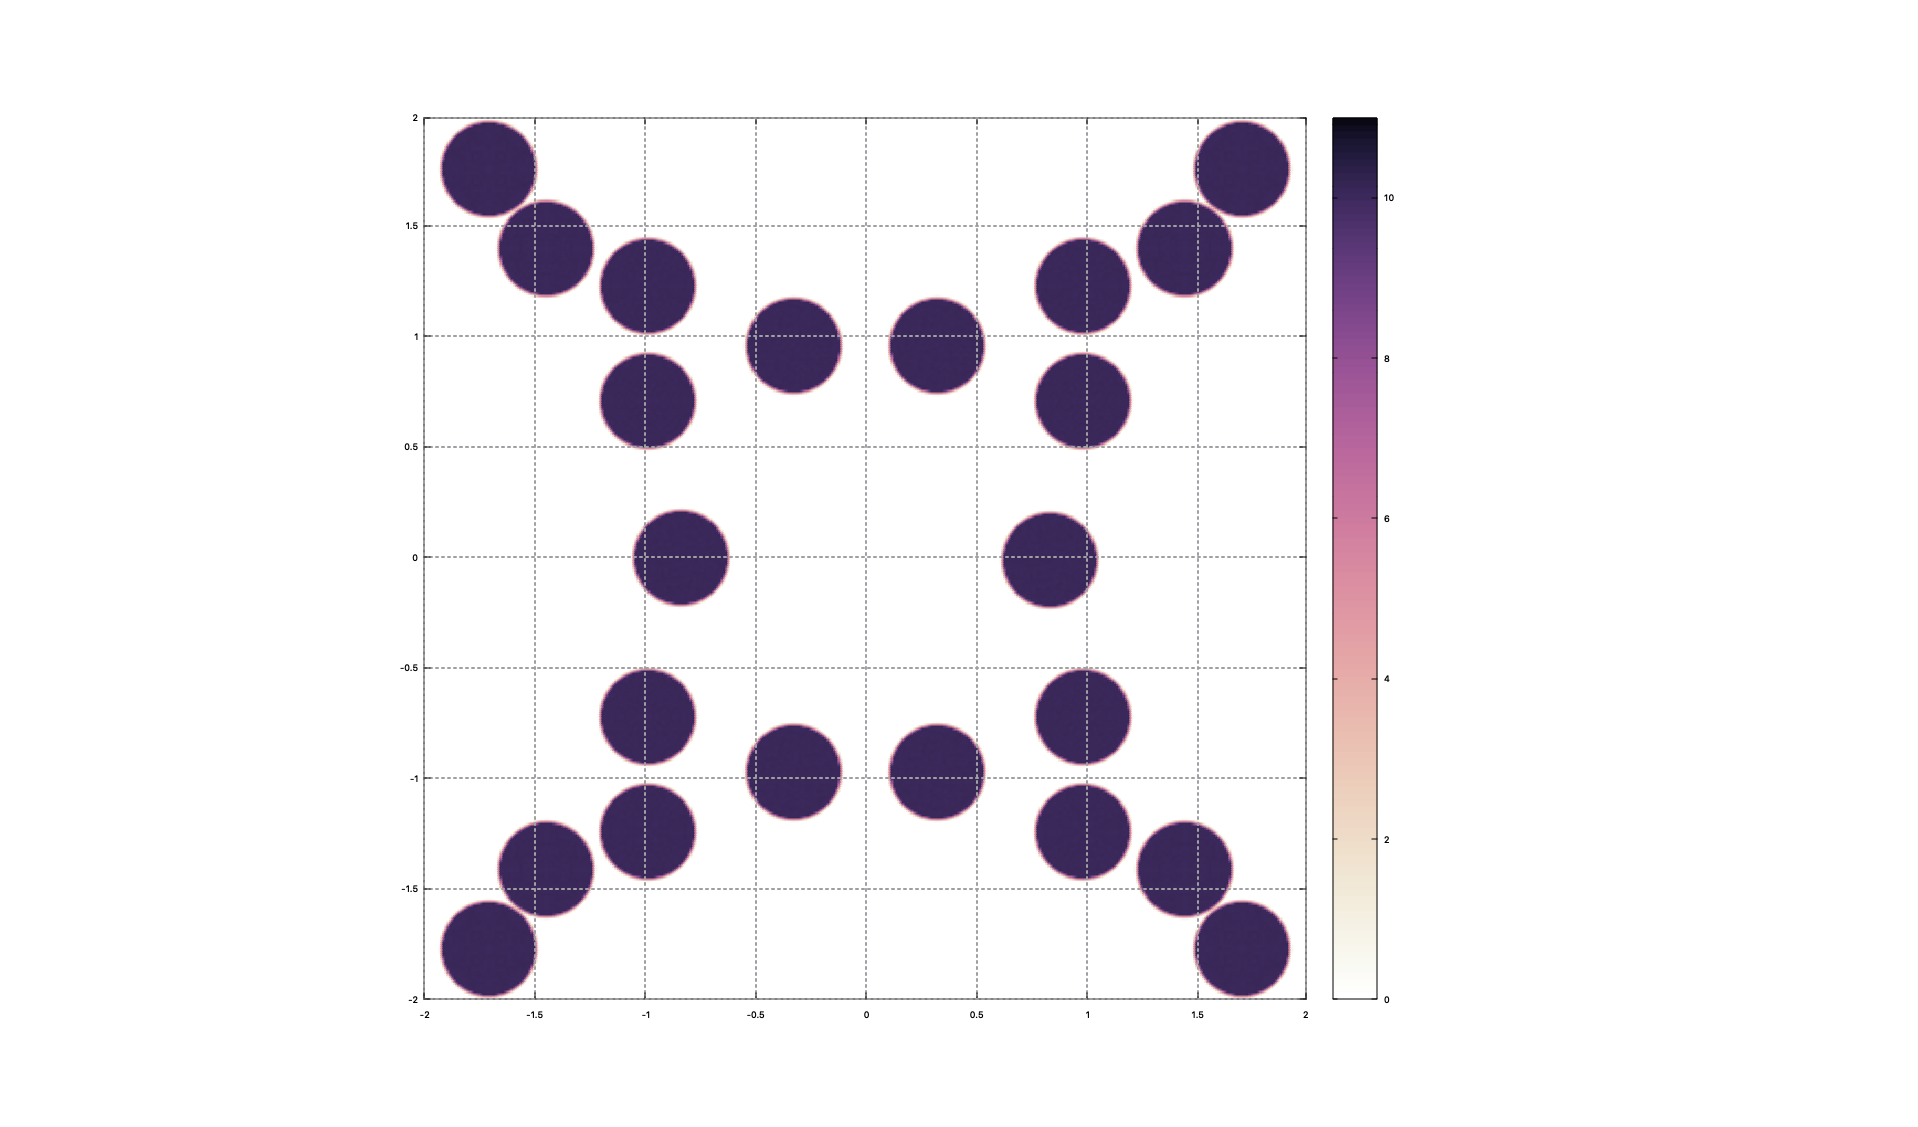
\includegraphics[width=4cm]{fig/GR30N90K30E2.png}
      \captionof{figure}{$a=30$}
    \end{column}
  \end{columns}


\end{frame}

\begin{frame}{数値計算例:楕円形のコアの回復 ポテンシャル観測}
  質点の数$K=30$,観測点数$N=90$とする.
  $a$は観測半径である.
  \begin{columns}
    \begin{column}{0.38\columnwidth}
      \setcounter{figure}{5}
      \centering
      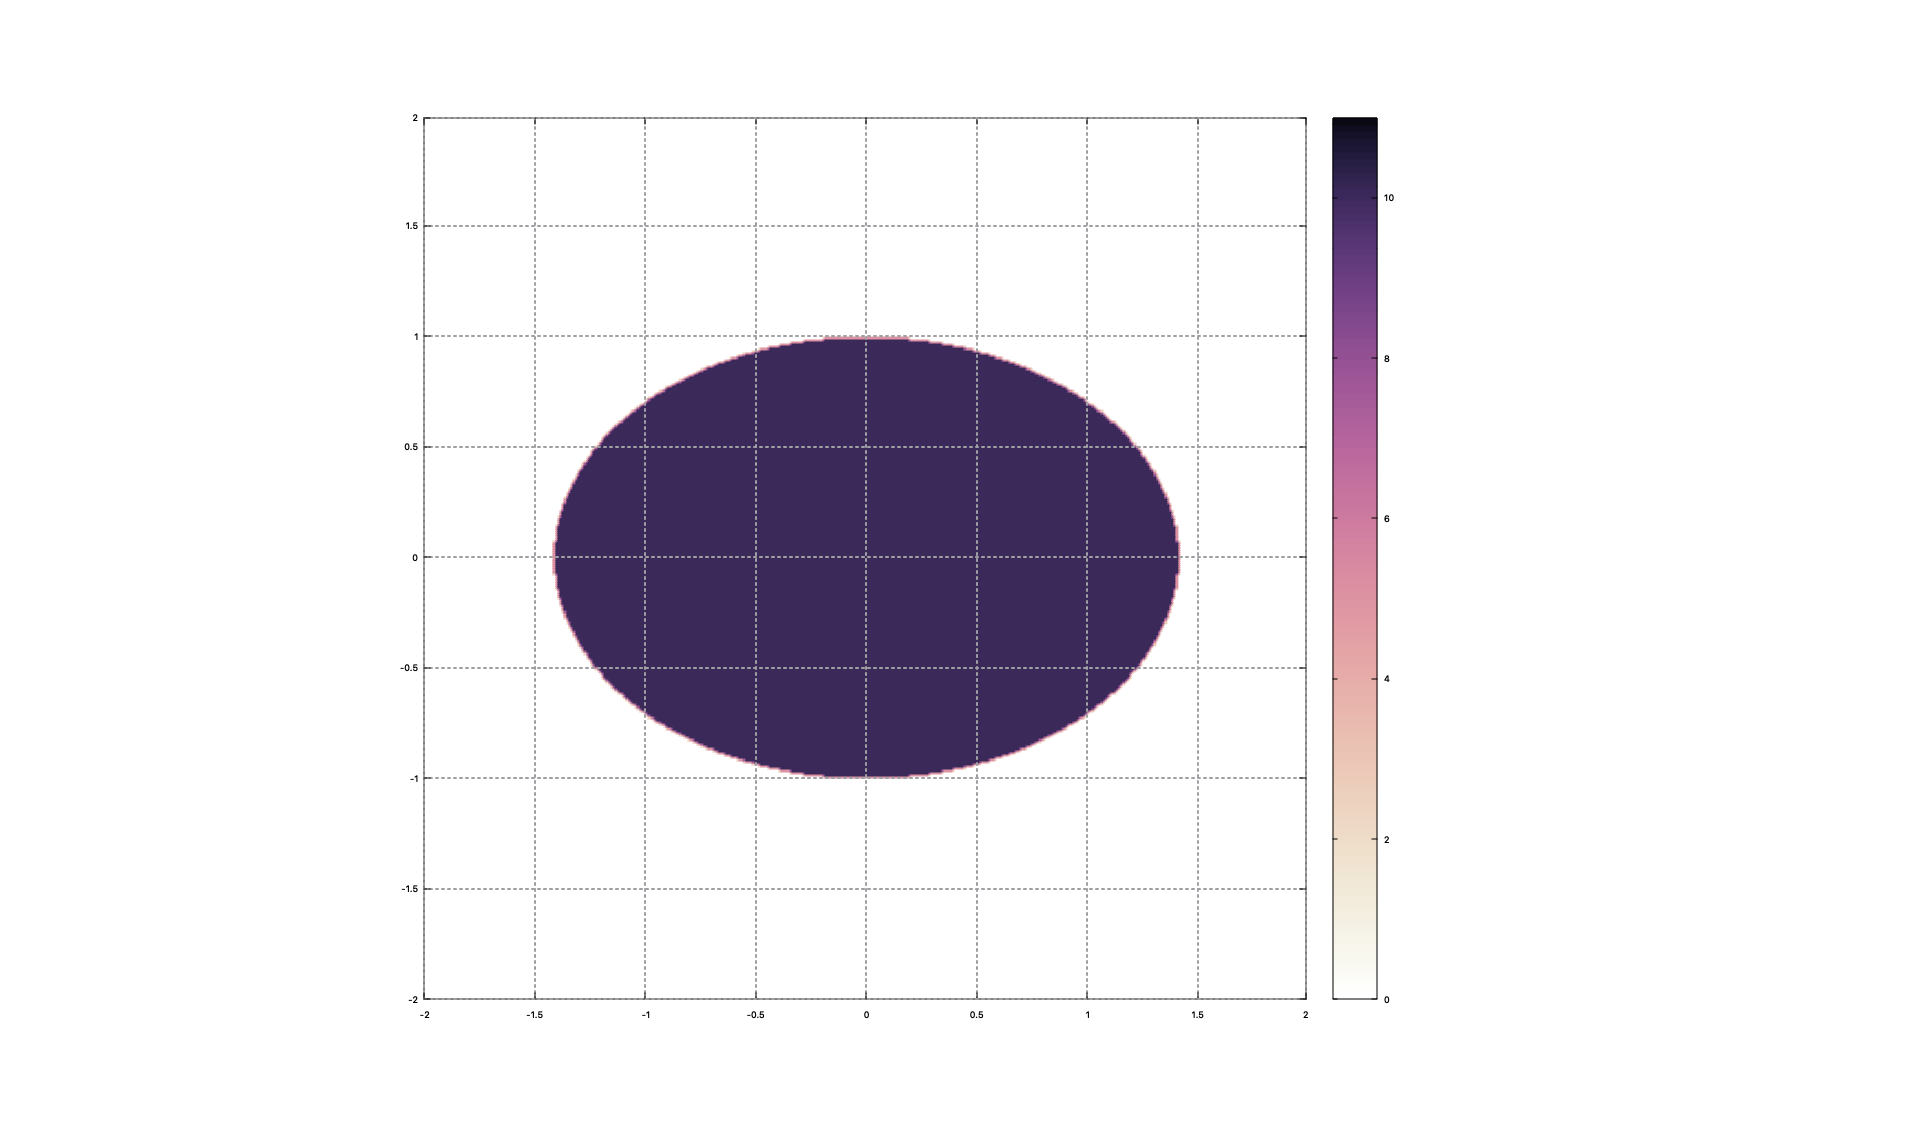
\includegraphics[width=4cm]{fig/elliptic.png}
      \captionof{figure}{厳密解}
    \end{column}
    \hspace{-1cm}
    \begin{column}{0.38\columnwidth}
      \setcounter{figure}{9}
      \centering
      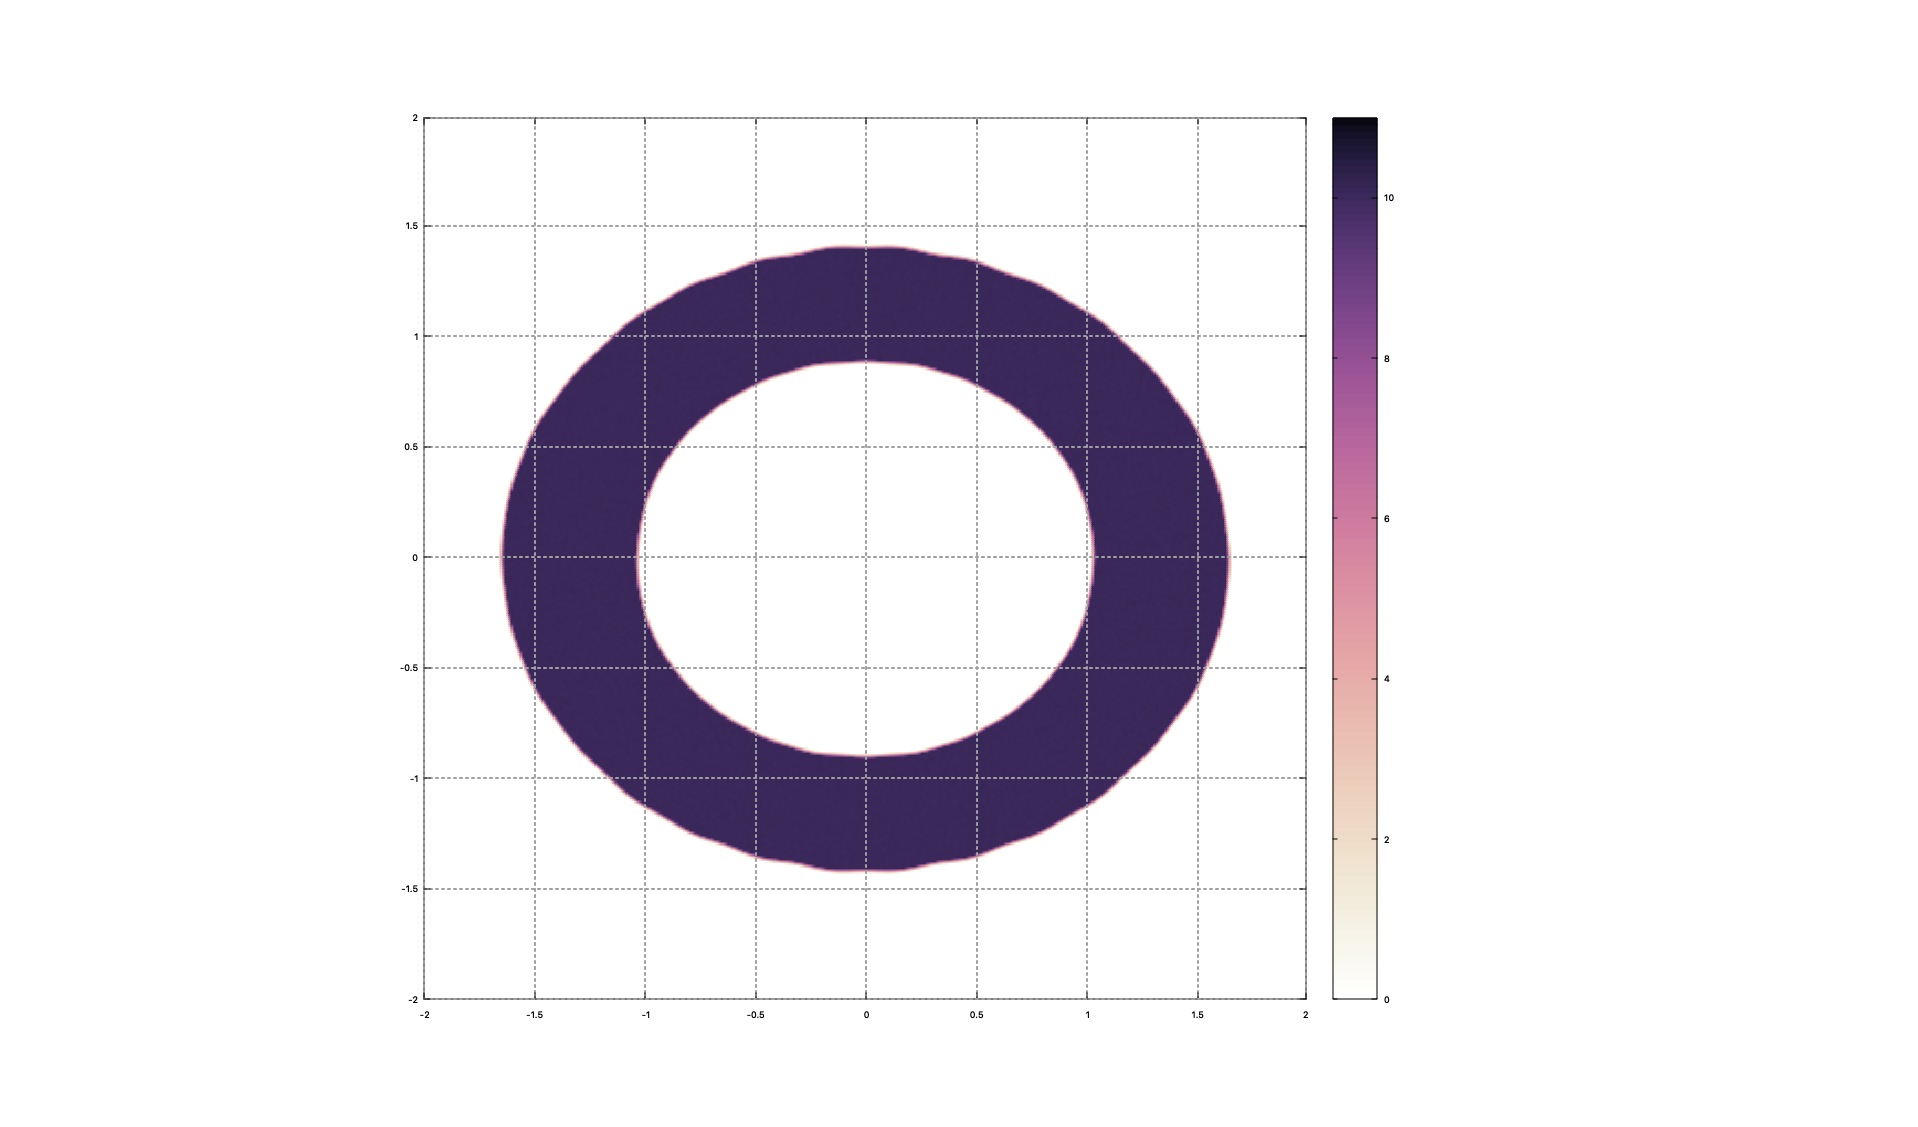
\includegraphics[width=4cm]{fig/PR4N90K30E2.png}
      \captionof{figure}{$a=4$}
    \end{column}
  \end{columns}

  \begin{columns}
    \begin{column}{0.38\columnwidth}
      \centering
      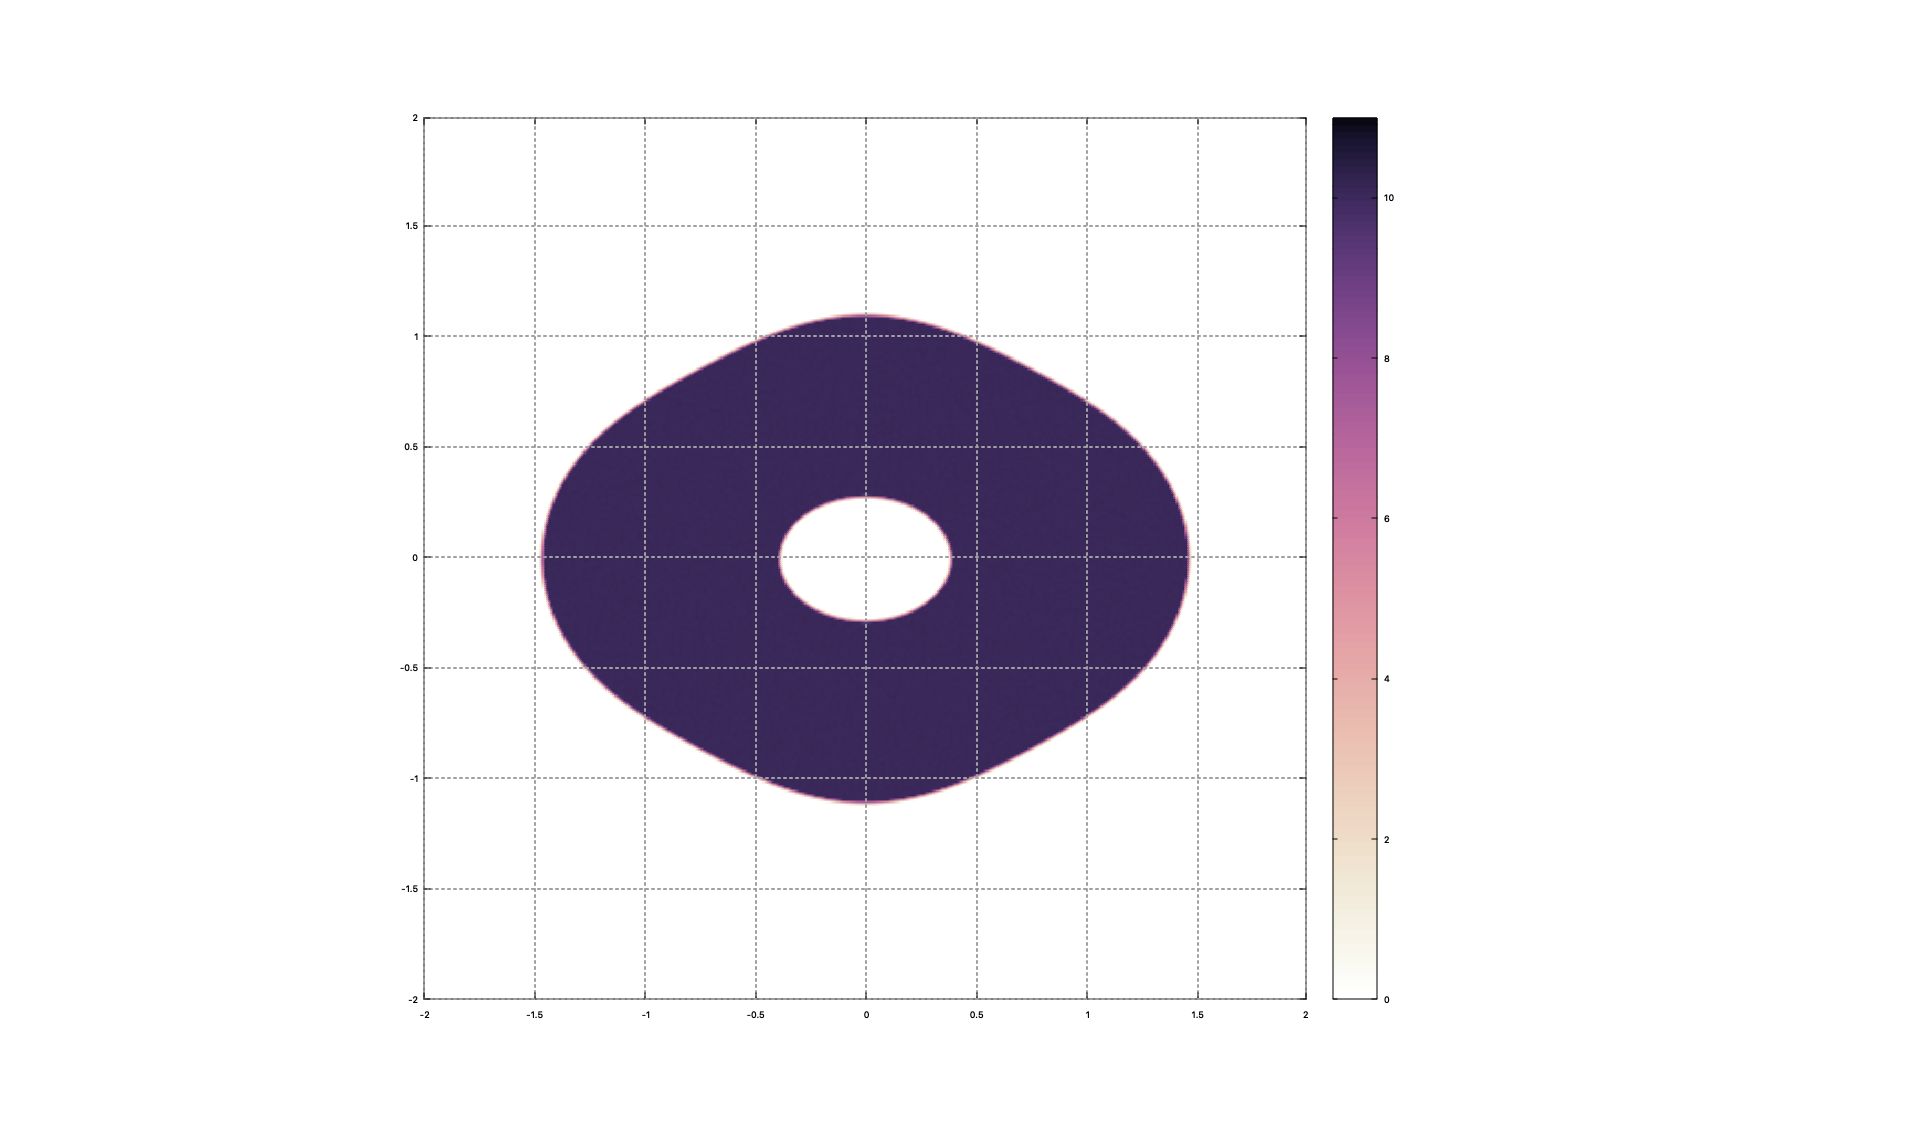
\includegraphics[width=4cm]{fig/PR10N90K30E2.png}
      \captionof{figure}{$a=10$}
    \end{column}
    \hspace{-1cm}
    \begin{column}{0.38\columnwidth}
      \centering
      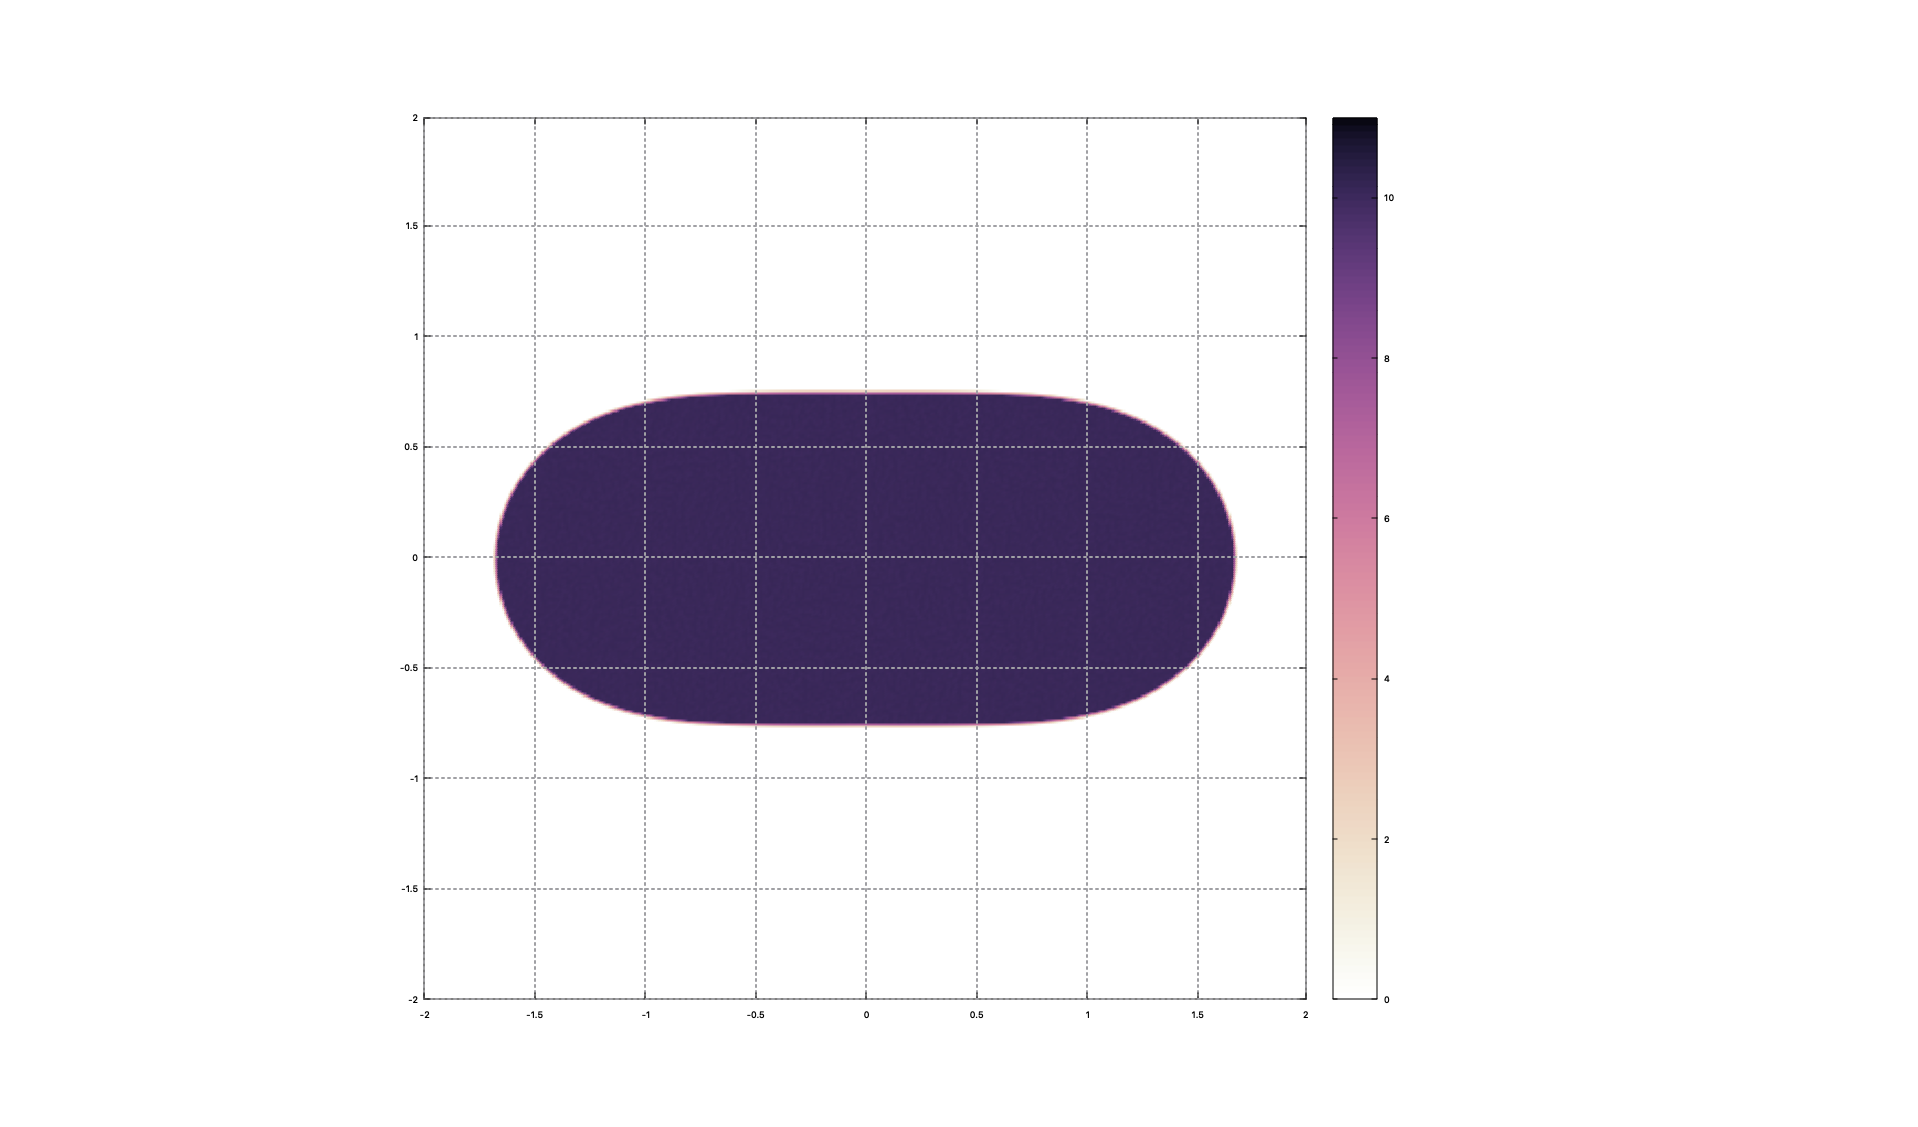
\includegraphics[width=4cm]{fig/PR30N90K30E2.png}
      \captionof{figure}{$a=30$}
    \end{column}
  \end{columns}

\end{frame}


\begin{frame}{結論}

  ポテンシャル逆問題において,境界でポテンシャルを既知とする問題設定を行い,重力を既知とする場合と比較して数値計算を行った.

  \begin{itemize}

    \item 楕円形のコアの回復

    重力観測と比べてポテンシャル観測の方がよりよい回復が望める.
  \end{itemize}

\end{frame}

\begin{frame}{参考文献}
  \begin{thebibliography}{99}
    \bibitem{An}
    G.Anger, 
    \textit{Inverse Problems in Differential Equations},
    Plenum Press,
    1990.
  
  
    \bibitem{Kr}
    R.Kress,
    \textit{Numerical Analysis},
    Springer,
    1998.
  
    \bibitem{No}
    野崎京三,
    『原子時計をセンサーとした重力ポテンシャル計の可能性』,
    応用地質技術年報,30号(2011),65-71.
  
    \bibitem{Sa}
    佐々木晶,
    『惑星内部構造』,
    地震,61巻特集号(2009),285-296.
  
  
    \bibitem{Za}
    L.Zalcman,
    Some Inverse Problems of Potential Theory,
    \textit{Contemporary Mathematics}, Vol.63(1987), 337-339.
  
    \bibitem{Zi} 
    D.Zidarov, 
    \textit{Inverse Gravimetric Problem in Geoprospecting and Geodesy},
    Elsevier,
    1990.
  \end{thebibliography}

\end{frame}

\end{document}
